\documentclass[tikz,border=8pt]{standalone}
\usepackage{amsmath,amssymb,bm}
\usepackage{sansmath}
\usepackage{tikz}
\usetikzlibrary{arrows.meta,calc}
\usepackage{pgfplots}
\pgfplotsset{compat=1.16}
\usepgfplotslibrary{groupplots}
\definecolor{cteal}{HTML}{2F5D62}\definecolor{cred}{HTML}{A44A3F}\definecolor{cochre}{HTML}{B08A45}
\definecolor{cgray}{HTML}{666360}\definecolor{clgray}{HTML}{9A9791}\definecolor{csage}{HTML}{7D9D8C}
\definecolor{cpurple}{HTML}{7A5B78}\definecolor{cdark}{HTML}{3B3A38}\definecolor{cmid}{HTML}{8E8B85}\definecolor{cpaper}{HTML}{F6F4F0}
\pgfplotsset{paper/.style={font=\sffamily\sansmath\scriptsize, axis line style={black!65,line width=0.4pt},
  tick style={black!65,line width=0.4pt}, tick align=outside, major tick length=2pt,
  axis x line*=bottom, axis y line*=left, grid style={line width=0.3pt,black!10},
  legend style={draw=none,fill=none,font=\sffamily\sansmath\scriptsize}, legend cell align=left,
  title style={font=\sffamily\sansmath\scriptsize,at={(0,1)},anchor=south west,yshift=3pt,xshift=-2pt},
  label style={font=\sffamily\sansmath\scriptsize}, ticklabel style={font=\sffamily\sansmath\scriptsize},
  yticklabel style={font=\sffamily\sansmath\scriptsize}, xticklabel style={font=\sffamily\sansmath\scriptsize}}}


\newcommand{\logit}{\operatorname{logit}}\newcommand{\expit}{\operatorname{expit}}
\begin{document}
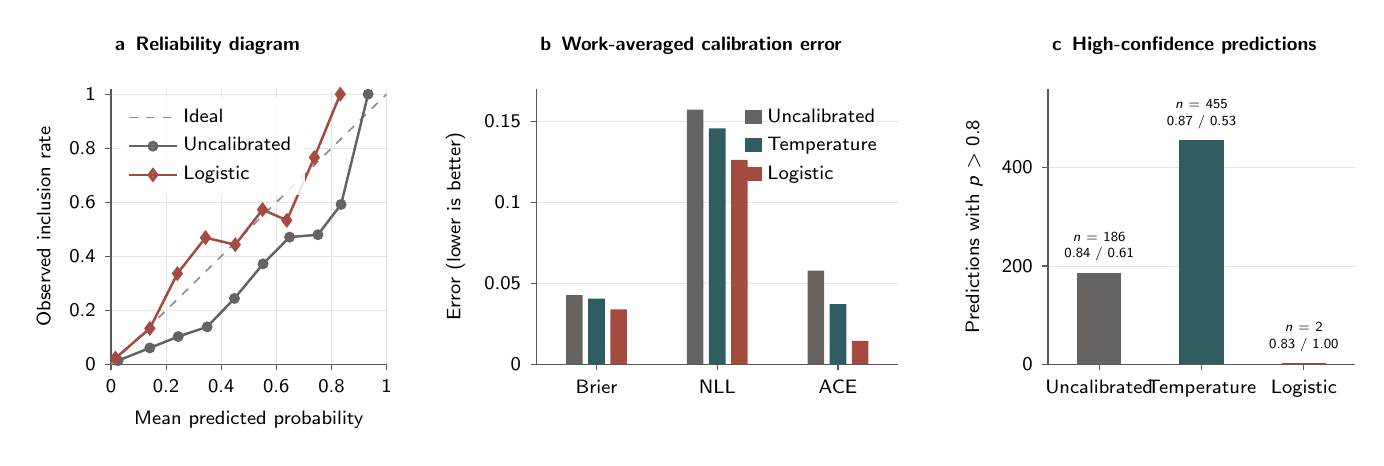
\begin{tikzpicture}
\begin{axis}[paper, at={(0.9cm,0)}, scale only axis, width=3.5cm, height=3.5cm,
  xmin=0, xmax=1, ymin=0, ymax=1.02, xtick={0,0.2,0.4,0.6,0.8,1}, ytick={0,0.2,0.4,0.6,0.8,1},
  xticklabel style={/pgf/number format/fixed}, yticklabel style={/pgf/number format/fixed},
  xlabel={Mean predicted probability}, ylabel={Observed inclusion rate}, grid=major,
  title={\textbf{a}\enspace\textbf{Reliability diagram}},
  legend style={at={(0.03,0.97)},anchor=north west,cells={anchor=west},fill=white,fill opacity=0.85,text opacity=1}]
\addplot[black!45,dashed,line width=0.6pt] coordinates {(0,0) (1,1)};
\addplot[color=cgray,mark=*,mark size=1.5pt,line width=0.9pt] coordinates {(0.026,0.014) (0.141,0.061) (0.244,0.103) (0.349,0.139) (0.448,0.244) (0.552,0.372) (0.648,0.471) (0.751,0.480) (0.835,0.592) (0.933,1.000)};
\addplot[color=cred,mark=diamond*,mark size=2pt,line width=0.9pt] coordinates {(0.016,0.023) (0.141,0.133) (0.241,0.336) (0.343,0.469) (0.451,0.443) (0.550,0.573) (0.638,0.533) (0.738,0.766) (0.832,1.000)};
\legend{Ideal,Uncalibrated,Logistic}
\end{axis}
\begin{axis}[paper, at={(6.3cm,0)}, scale only axis, width=4.6cm, height=3.5cm,
  ybar, bar width=6pt, ymin=0, ymax=0.17, symbolic x coords={Brier,NLL,ACE}, xtick=data, enlarge x limits=0.25,
  yticklabel style={/pgf/number format/fixed,/pgf/number format/precision=2}, ylabel={Error (lower is better)}, ymajorgrids,
  title={\textbf{b}\enspace\textbf{Work-averaged calibration error}},
  legend style={at={(0.98,0.97)},anchor=north east,cells={anchor=west}}, legend image code/.code={\draw[#1,draw=none] (0cm,-0.08cm) rectangle (0.22cm,0.1cm);}]
\addplot[fill=cgray,draw=none] coordinates {(Brier,0.0427) (NLL,0.1572) (ACE,0.0579)};
\addplot[fill=cteal,draw=none] coordinates {(Brier,0.0406) (NLL,0.1456) (ACE,0.0371)};
\addplot[fill=cred,draw=none] coordinates {(Brier,0.0340) (NLL,0.1262) (ACE,0.0145)};
\legend{Uncalibrated,Temperature,Logistic}
\end{axis}
\begin{axis}[paper, at={(12.8cm,0)}, scale only axis, width=3.9cm, height=3.5cm,
  ybar, bar width=16pt, ymin=0, ymax=560, symbolic x coords={Uncalibrated,Temperature,Logistic}, xtick={Uncalibrated,Temperature,Logistic}, enlarge x limits=0.25,
  ylabel={Predictions with $p>0.8$}, ymajorgrids, title={\textbf{c}\enspace\textbf{High-confidence predictions}}]
\addplot[fill=cgray,draw=none,bar shift=0pt] coordinates {(Uncalibrated,186)};
\addplot[fill=cteal,draw=none,bar shift=0pt] coordinates {(Temperature,455)};
\addplot[fill=cred,draw=none,bar shift=0pt] coordinates {(Logistic,2)};
\node[font=\sffamily\sansmath\tiny,align=center,anchor=south] at (axis cs:Uncalibrated,190) {$n=186$\\0.84 / 0.61};
\node[font=\sffamily\sansmath\tiny,align=center,anchor=south] at (axis cs:Temperature,459) {$n=455$\\0.87 / 0.53};
\node[font=\sffamily\sansmath\tiny,align=center,anchor=south] at (axis cs:Logistic,6) {$n=2$\\0.83 / 1.00};
\end{axis}
\end{tikzpicture}
\end{document}
